\section{Materials and Methods}

    This project will analyze a system of two, two dimensional, rigid, tandem foils and a downstream pressure array, as depicted in \Fref{fig:methods:2D Setup}. It is broken down into a series of smaller objectives which will build in complexity and provide data for the subsequent steps.

\subsection{Experimental Setup}
\subsubsection{Tandem Foils}
%% Figure out who's making a fin and what it will be made of
     The tandem foil setup will mirror that of \citep{Boschitsch2014} so that data can be easily compared. The foils will be made from aluminum and have a NACA0016 cross section with a chord length, \(C\), of 8 cm. The NACA0016 foil will lend itself to better inferences between data, as its characteristics are well documented and understood. The foil spacing, \(S\), will be fixed at one chord length, so that the downstream foil will not influence the upstream foil's vortex formation. The foils will pitch about points one quarter chord length behind their leading edges. To make this project attainable using USNA equipment, the foils will not undergo heave motions. This should not change vortex formation or interactions. Their equations of motion are shown in Table 1, and are further explained in Section 1.2. The fins will flap at \(St=0.25\) with \(A=0.25C\) and \(\theta_m=15\deg\), similar to the movements in \citep{Boschitsch2014}.

\begin{table}
\caption{Equations of Foil Motion}
\label{tab:methods:EOM}
\begin{center}
\begin{tabular}{ccc}
\toprule
Motion & Upstream Foil & Downstream Foil \\ 
\midrule
Pitch & \(\theta(t)=\theta _msin(\omega t)\) & \(\theta (t)=\theta _msin(\omega t+\phi)\) \\
\end{tabular}
\end{center}
\end{table}
\begin{figure}
\begin{center}
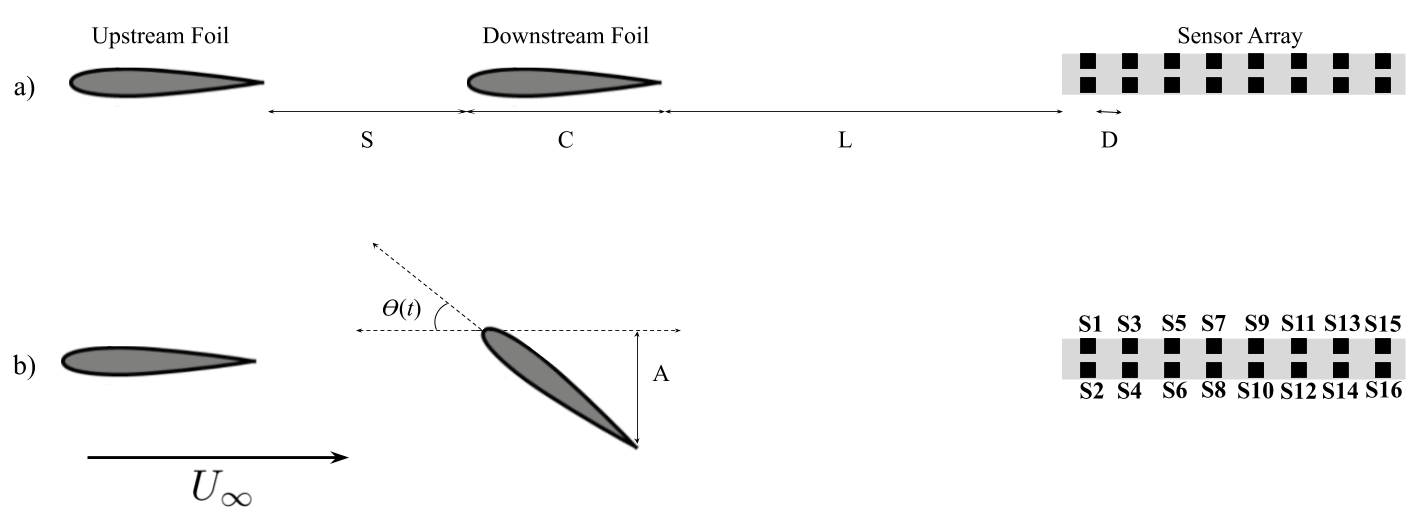
\includegraphics[width=0.8\columnwidth]{figures/Experimental Setup.png}
\end{center}
\caption{Stationary depiction of 2D tandem foil experiment setup with foil spacing, chord length, and sensor spacing marked (a). 2D tandem foils in motion with foil pitch angle, stroke amplitude, and free stream velocity marked (b).}
\label{fig:methods:2D Setup}
\end{figure}

\subsubsection{Pressure sensor array}

    The pressure sensor array will consist of six MS5407-AM sensors from Measurement Specialties. These sensors will be arranged into two rows on opposite sides of a PVC pipe, as shown in \Fref{fig:methods:2D Setup}, with spacing, \(D\), of 2 cm. The surface of each pressure sensor is waterproof. The sensors will contact the water through drilled holes in the surface of the pipe, and the space between the walls of the pipe and the rims of the sensors will be caulked against the outside water. Sensor readings will feed into a Hewlett Packard Elitebook via a Wheatstone Bridge setup and an ARM Mbed microprocessor. This configuration is inspired by that of \citep{Venturelli2012}, and will achieve a sampling frequency of 50 Hz.
% Cam 12/30: could also use the W106B51/-0002 sensors available in the hydro lab, although it would be best to have about twice as many for the purpose of being able to take differential pressures across the pipe at several locations

\subsubsection{Flow Parameters}

    For comparison with \citep{Muscutt2017}, the free stream velocity, \(U_\infty\), will be 0.06 m/s.
% Cam 12/31: include discussion of Reynolds number for the fins?

\subsection{Simulation of Tandem Fins}

    A physical sensor array will be affected by noise and drift, so it will be beneficial to simulate the experiment so that expected results can be compared with the actual results. Additionally, the simulated experiment can be run quickly at any location, and is excellent for generating a large amount of sample data. The experimental setup described in Section 4.1 will be replicated in Lily Pad using the Boundary Data Immersion Method (BDIM) with 64 grid points per chord length. The setup will mirror that of \citep{Muscutt2017}, and the pressure at the sensors marked in \Fref{fig:methods:2D Setup} will be recorded.

% mention that simulation will be validated by doing just 1 foil first and comparing results to another person?

    The simulation will run 30 times with two fin oscillations per trial. The phase angle, \(\phi\), will range from 0 to 180°. Every fifth trial's data will be set aside to form the test data for the wake classifier. The remaining 24 trials' circulation plots will be inspected visually to determine the mode of wake interaction, and the data will be sorted into categories for constructive, destructive, and paired vortex interactions. These trials will constitute the truth data for training the wake classifier.

\subsubsection{Feature Extraction}
    
    The differential pressures between vertical sensor pairs (e.g. s1 - s2) and the differential pressures between horizontal pairs (e.g. s1 - s3) will be plotted against time in Matlab. This will show the sensor array's expected response to a complex vortex wake, while also presenting an opportunity for feature selection. Numeric traits that differentiate the three modes of wake interaction will be selected based on these plots. The traits calculated in previous studies will serve as a starting point.
    
    The Fast Fourier Transform (FFT) has determined the vortex shedding frequency based on pressure signals on a lateral line \citep{Venturelli2012}. In the presence of paired vortices, the FFT should yield multiple dominant frequencies. The frequency corresponding to the vortex shedding will be low, while the frequency corresponding to the space between two paired vortices should be high. In the presence of constructive or destructive vortex interactions, the FFT should yield a single frequency, making this a salient feature for differentiating the paired vortex wake from the other two modes.
    
    Other features will be calculated as ratios between measured qualities, which should achieve robustness over the entire set of possible data. These features may include ratios that express the average peak differential pressure, the rise time, or fall time.
    
\subsubsection{Wake Classification}

    The features calculated in Section 4.2.1 will be arranged into a classification matrix in Matlab according to the format shown in \Fref{fig:methods:Class Matrix}. Each type of feature will be grouped into the same column, while each feature for a particular trial will be placed in the same row. The rows will be given truth data as numbers, where '1' indicates constructive vortex wakes, '2' indicates paired vortex wakes, and '3' indicates destructive vortex wakes. The second column will be the label assigned by the classifier during training, and its initial values will be 1. 
    
    The Bayesian classifier and the multilayer perceptron (MLP) functions in Matlab will both be used to train networks on the classification matrix. The accuracy and confusion matrices for both classifiers will be compared to determine the most accurate method.
    % describe the data analysis in future section and reference here

\begin{figure}
\begin{center}

\includegraphics[width=0.75\columnwidth]{figures/Classification Matrix.png}
\end{center}
\caption{Classification matrix with n features to be used for training a system to identify wakes.}
\label{fig:methods:Class Matrix}
\end{figure}

% Cam 12/31: section on determining phase shift?

\subsection{Experimental Test of Flapping Foils}

    The physical sensor array must be calibrated before physically replicating the tandem fin experiment. The array configuration is described in Section 4.1.2.
    
\subsubsection{Sensor Calibration} \label{Sensor Calibration}

    Each sensor is impacted by noise and bias drift, which cause high and low frequency disturbances to the output data, respectively. While noise is random for each sensor, the bias of each unit is unique and due to small errors in manufacturing. To overcome the bias, each sensor will be calibrated simultaneously in still water over the course of five minutes. A combination of high and low pass filters will produce a bandpass filter that will minimize the effects of bias and noise.
    
    The frequency of the bias drift will be found for each sensor, and digital high pass filters will be designed for each sensor and implemented on the Mbed microprocessor using Tustin's transform. They will be of the form \[x_n=\frac{2-aT}{2+aT}x_n_-_1+\frac{2}{2+aT}(y_n+y_n_-_1)\] where \(x_n\) and \(x_n_-_1\) are the current and previous output reading, respectively, \(y_n\) and \(y_n_-_1\) are the current and previous input readings, respectively, \(T\) is the sampling period, and \(a\) is the cutoff frequency to be varied. The sampling period is related to the sampling frequency by \(T=\frac{1}{f}=\frac{1}{50}\sec\). The cutoff frequency for a given sensor will be the experimentally derived bias frequency.
    
    In a similar manner, digital low pass filters will be applied to the sensor output to reduce the effects of noise. The cutoff frequency will be the highest frequency observed in the tandem fin simulation. The low pass filters will be of the form \[x_n=\frac{2-aT}{2+aT}x_n_-_1+\frac{aT}{2+aT}(y_n+y_n_-_1)\]

\subsubsection{Experiment Setting} \label{Experiment Setting}

    A single flapping fin and the sensor array will be placed in the Large Re-Circulating Flow Tank located in the Naval Academy Hydrodynamics Laboratory, with dimensions 0.41 m x 0.41 m x 1.50 m. The tank will be driven by a four-bladed axial flow impeller to achieve a uniform flow speed of 0.06 m/s.

\subsubsection{Mechanical fin} \label{Mechanical fin}

    The mechanical fins employed for this objective will be plastic replicas of a mola mola (ocean sunfish) dorsal fin, previously built for research projects within the Biomechanics Laboratory. The fins will be the same height as the flow tank, which will minimize 3D flow effects and create a response that is well represented by the 2D simulation. The fins will each be actuated by two RC servo motors, whose responses will be controlled by means of a raspberry pi. The fin equations of motion described in Section 4.1.2 will be implemented on the raspberry pi to actuate the fins in a manner identical to the simulations.

\subsubsection{Experimental Trial Procedure} \label{Experimental Trial Procedure}

    The tandem fins will flap for a series of fifteen trials at phase angles ranging from 0 to 180°. Each trial will begin at rest for 2 seconds,  the fins will flap for five cycles, and the system will come to rest for two additional seconds. The pressure readings during the first two seconds of the trial will show the noise and unperturbed water pressure. The constant pressure reading over the last two seconds will indicate any bias in the pressure readings over the course of the experiment. Keeping each trial short should further minimize the possibility of sensor drift, but if the pressure during the last two seconds is greater than 5\% different from the initial two, the trial will be discarded and repeated.

    The pressure data will be saved for further analysis. 
    
\subsubsection{Data Processing} \label{Data Processing}
    
    The differential pressure plots will be compared with those generated in Section 4.2.1 for simulation accuracy. If the pressure plots agree within 5\% error, the experimental data will be separated into two categories. Every third trial will be placed in a 'test data' category, and the remaining trials will make up the 'training data'. The classifier developed in Section 4.2.2 will be retrained with this additional training data. To make the system robust against noise, the experimental trial will be partitioned into 3 second segments, each of which will become another input for the classification matrix. The features developed in Section 4.2.1 will be calculated for each 3 second segment, and these will also be entered into the classification matrix. The classifier will be retrained using this data, and it will be tested on the data set aside earlier. The classifier developed will be incorporated into a program that approximates the wake interaction mode over three second intervals.

    
\subsubsection{Validation}

    The script developed in Section \ref{Data Processing} will be tested in real time using the setup in Section \ref{Experimental Trial Procedure}. The fins will be flapped for three trials, with each lasting thirty seconds. The first, second, and third trials will be run with phase difference of 0, 90°, and 180°, respectively. These phase angles should demonstrate each of the three wake interaction modes. The classifier output will be recorded for every three seconds and recorded for comparison.
